\chapter[Implementering af hardware]{Hardware}
\mnote{Nick Østergaard}

% Vi skriver her om hvordan vi faktisk realiserer det vi har sankket
% om i Hardwaredesignet

\section{Stepmotor driver}
\label{sc:stepmotor-driver}
\fixme{Omformuleres!}Vi skal konstruere en
stepmotor driver med et par integrerede stepmotor drivere. Mere
specefikt anvender vi et par L6208N'ere, som kan styre en bipolar
stepmotor. Vi bruger denne driver, da den er simpel at styre, samt der
er mulighed for at lave strømbegrænsning. Hvilket vil gøre, at vi kan
skrue forsyningsspændingen til motorerne op og begrænse strømmen,
således motorerne er mere kvik, hvilket betyder at vi kan køre
hurtigere.


\mnote{
  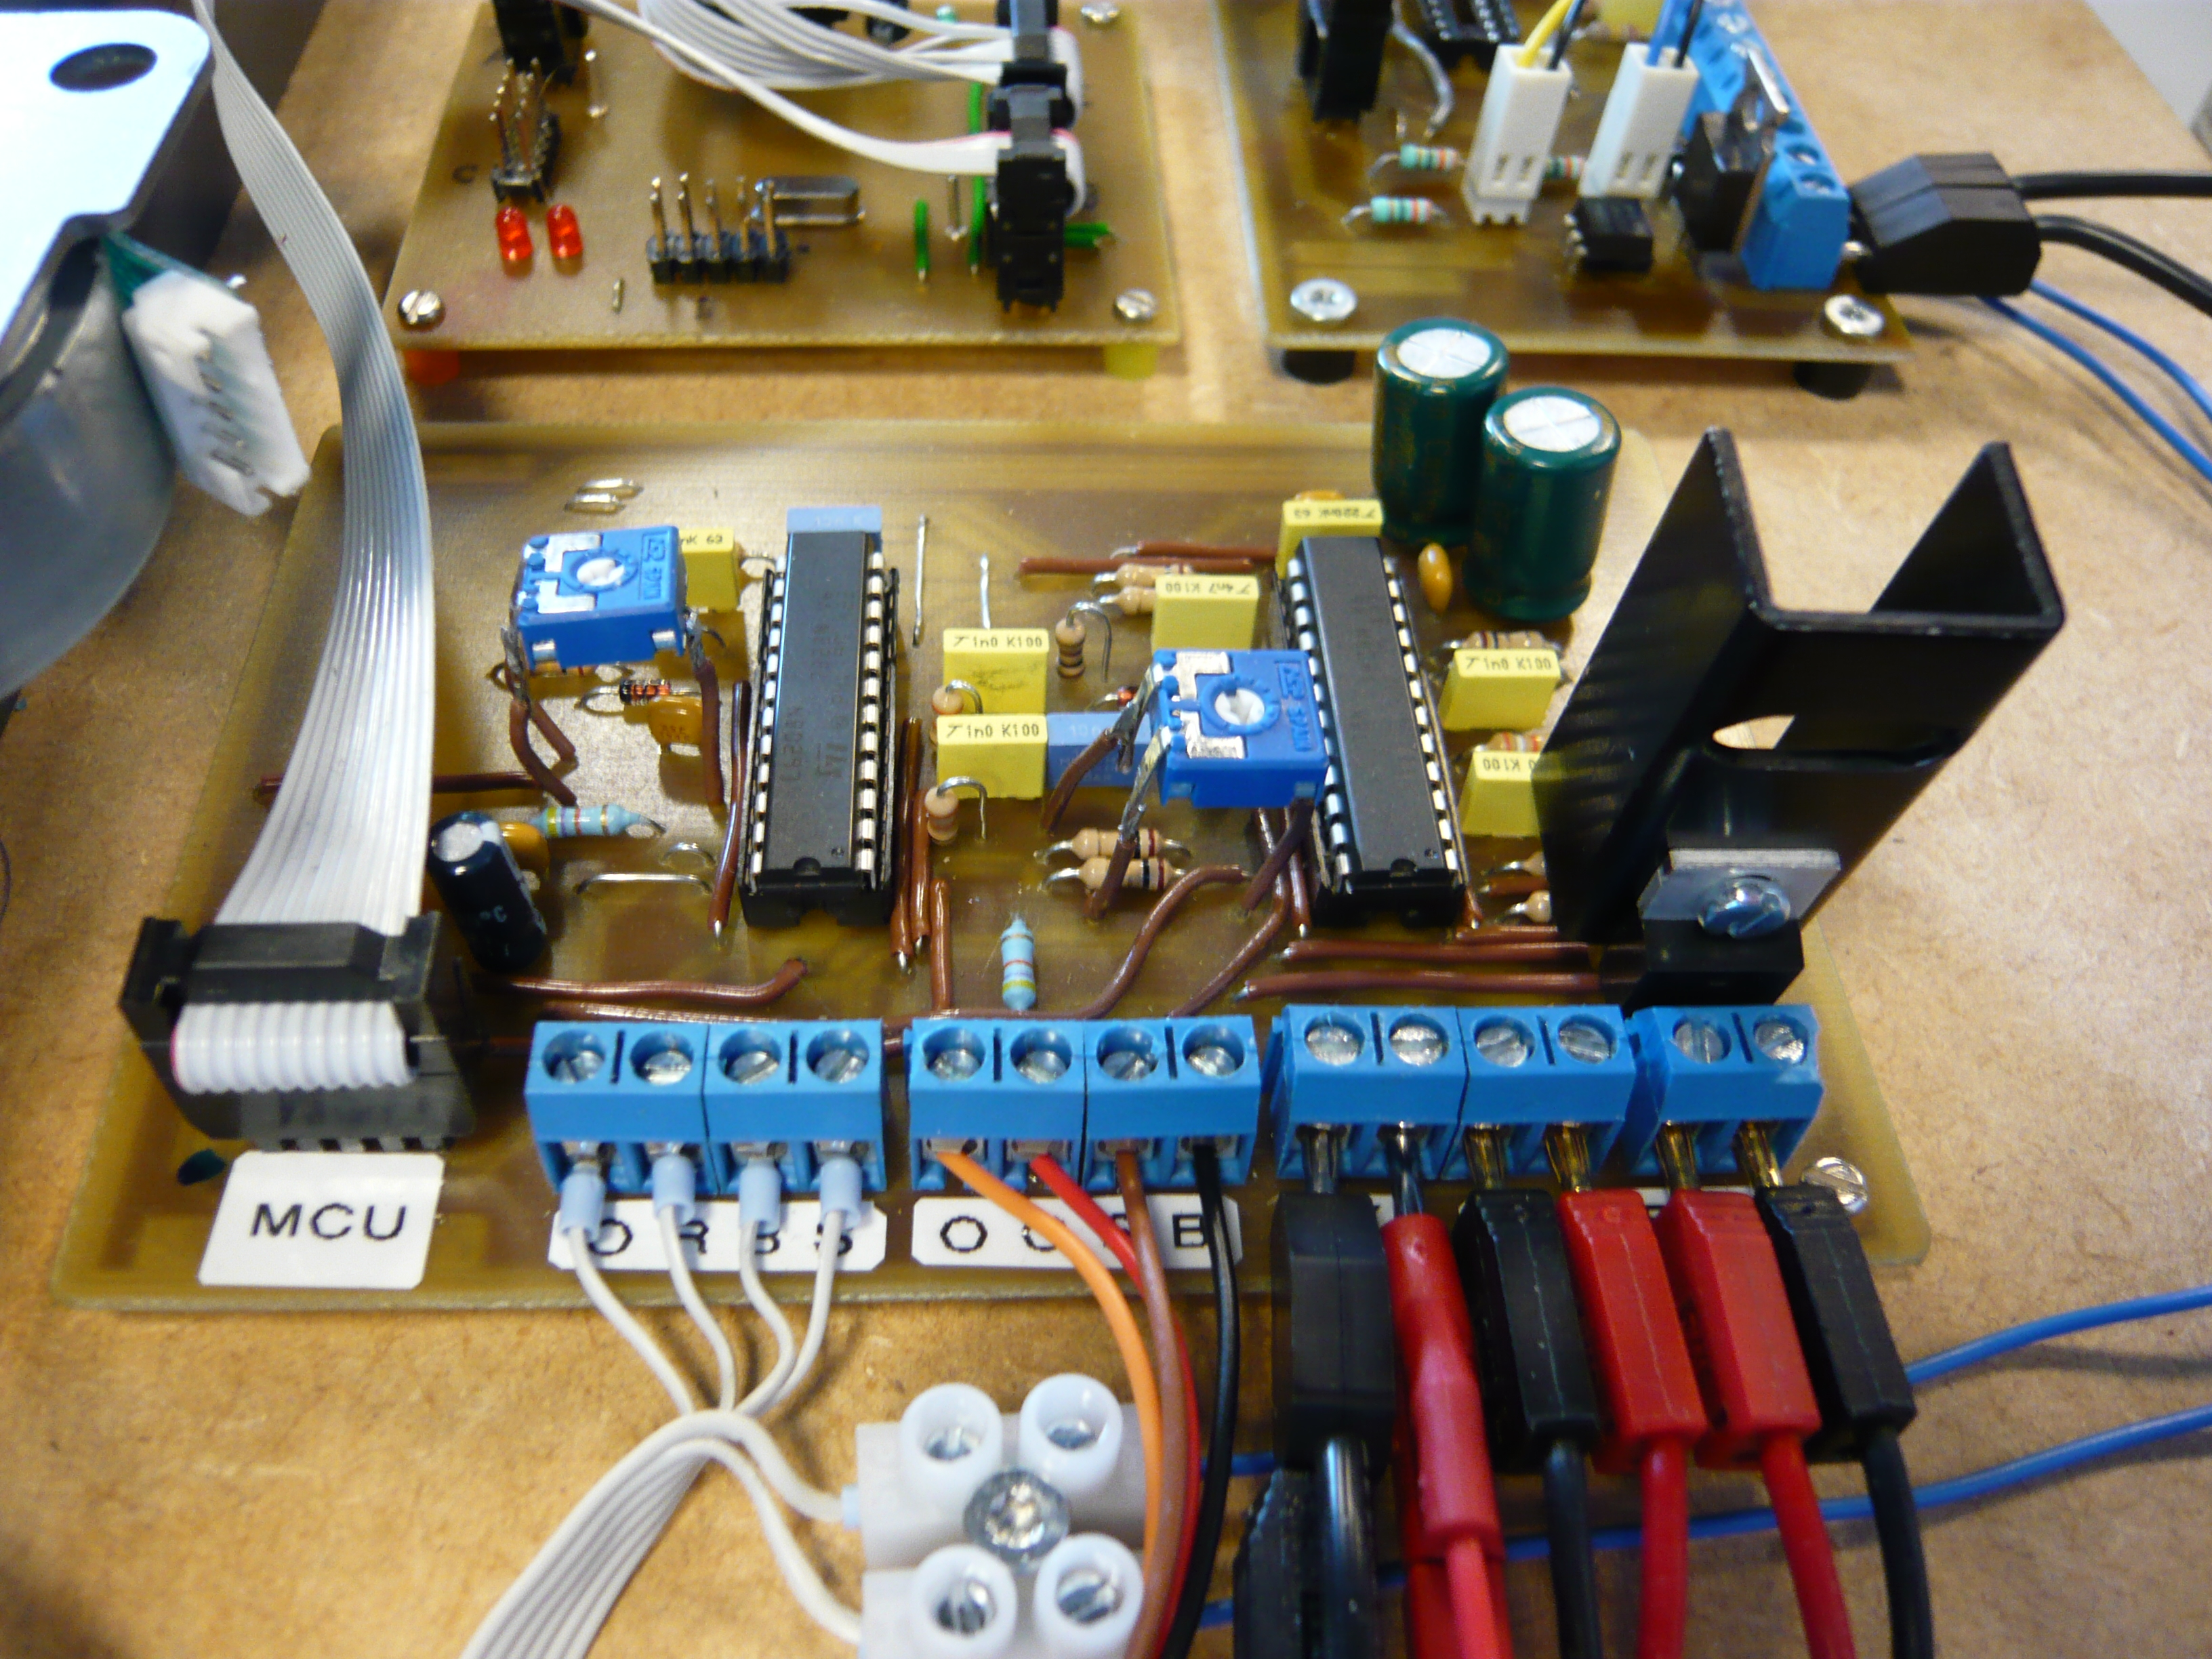
\includegraphics[width=\marginparwidth]{./img/stepmotordriver}
  \captionof{figure}{Stepmotor driver}
  \label{fig:stepdriver}
}
\fixme{Nick: Beskær billede}

\mnote{
  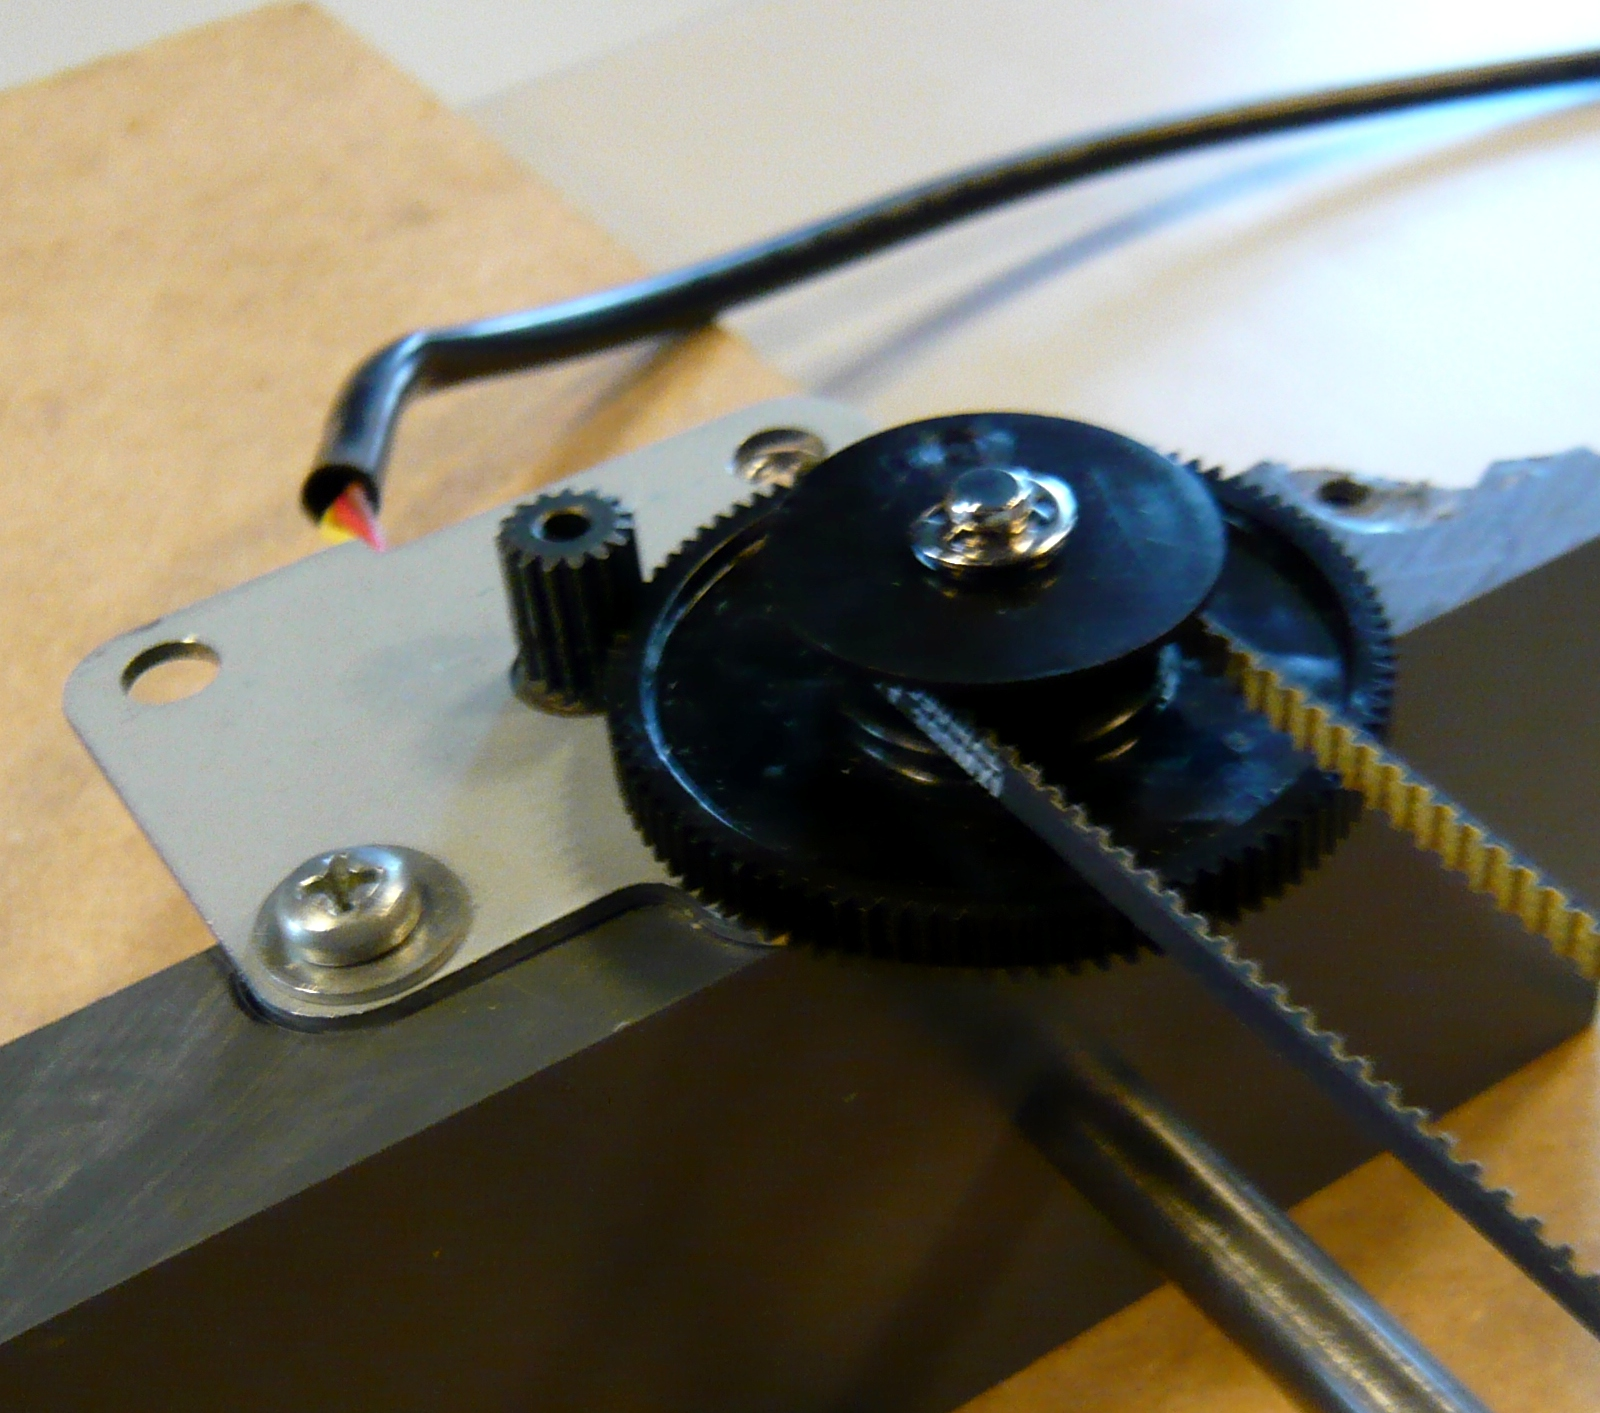
\includegraphics[width=\marginparwidth]{./img/x-motor}
  \captionof{figure}{X-aksens motor monteret}
  \label{fig:x-motorimg}
}

\mnote{
  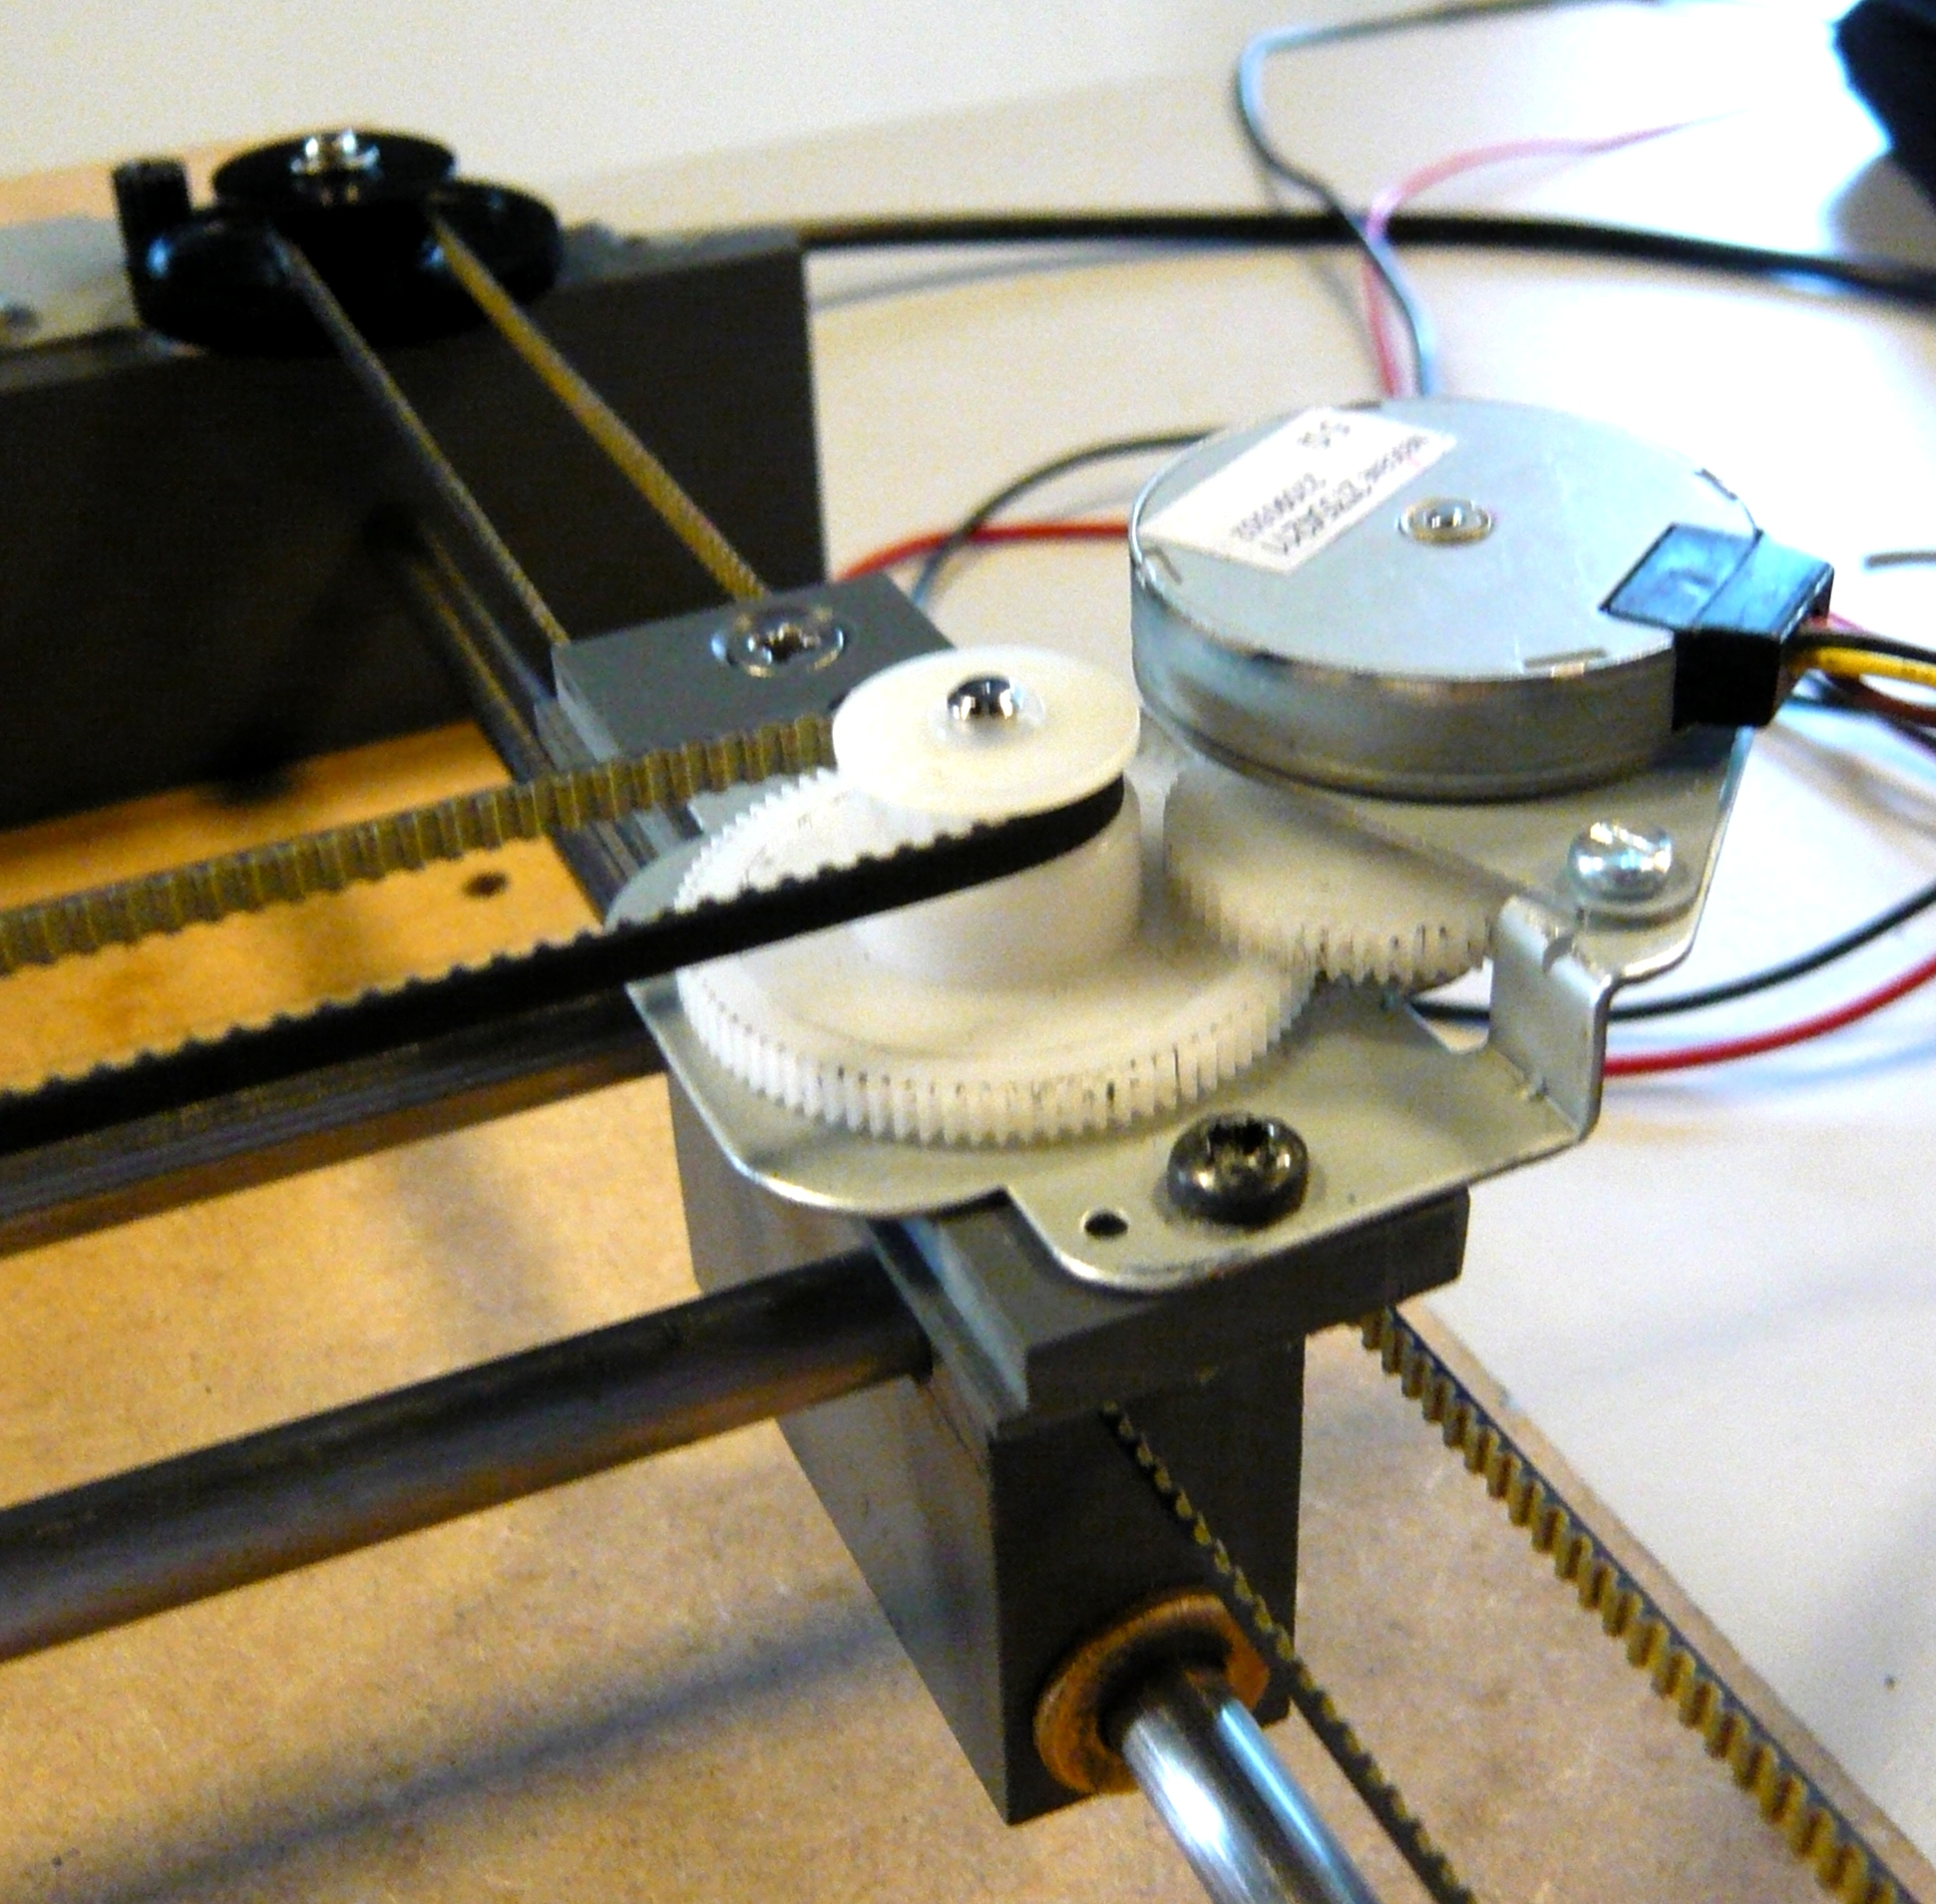
\includegraphics[width=\marginparwidth]{./img/y-motor}
  \captionof{figure}{Y-aksens motor monteret}
  \label{fig:y-motorimg}
}

\section{Sensorerne}
\fixme{delkredskøb til gaffelsensorerne}

\mnote{
  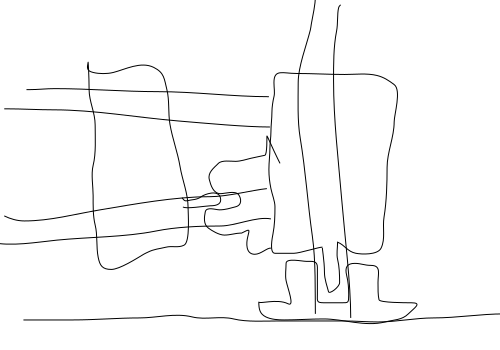
\includegraphics[width=\marginparwidth]{./img/fotogafel-skitse}
  \captionof{figure}{Placering af fotogafler}
  \label{fig:transducer-skitse}
}
\fixme{nick: Illustrationen af sensorerne skal laves rigtigt}

\mnote{
  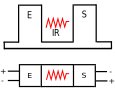
\includegraphics[width=\marginparwidth]{./img/fotogaffel}
  \captionof{figure}{Skitse af fotogaffel}
  \label{fig:fotogaffel-skitse}
}

\section{SD-kort adapter}
Som følge af at vi har bestemt i vores kravspecifikation, at vi skal kunne lægge data på et
SD-kort, og få poltteren til at tegne det vi har bestemt i dataene, så
skal vi selvfølgelig også have lavet en SD-kort adapter.

Vi har ved at kigge på litteratur \cite{web:captain-mmc} og
\cite{web:sd-pinout}, konstrueret en SD-kort adapter vi kan bruge til
vores ATmega128 print.

\fixme{Billede af SD-kort adapter}
\fixme{Printlayout og pinout}

\fixme{Beskriv kort, hvordan vi aktiverer vores sænker}

%%% Local Variables: 
%%% mode: latex
%%% TeX-master: "../master"
%%% End: 
